\documentclass[11pt,twocolumn]{article}
\usepackage{graphicx}
\usepackage{biblatex}

\addbibresource{main.bib}

\title{Consensus in the Browser using WebRTC}
\author{Blade Chapman}
\date{}

\begin{document}
\maketitle

\begin{abstract}
The traditional model for consensus-driven applications is to build a network of managed servers that vend a large number of clients. This centralization raises questions of privacy, data ownership, and reliability for the customers of these applications. This project explores the potential of achieving consensus on the end-user’s device as a means of addressing these questions. We do this by providing an implementation of the Raft consensus algorithm that can be run in the browser and communicate directly with peers via WebRTC. We then demonstrate this implementation with a simple chat application that uses Raft to achieve consensus on chat history. We find that using peer-to-peer channels for achieving consensus inherently protects the end user better than traditional architectures, but requires demanding guarantees on algorithm latency and ability to adapt to varying network conditions.\\
\end{abstract}

\section{Introduction}
As software products become more collaborative, achieving consensus has become a common problem amongst application developers. Customers use Facebook Messenger, Google Docs, and Dropbox's Shared Folders with the expectation that the data presented is up-to-date and visible by other collaborators. The traditional model for building these applications has been to service a large number of customer devices with a smaller set of administrated servers and data centers that do the work of propagating and persisting data. As evidenced by the popularity of the aforementioned products, this model has served the industry well and has proven performance and reliability characteristics.

However, recent events have sown doubt amongst customers' trust in these centralized entities. Companies whose business models depend on understanding their users thoroughly are not directly incentivized to provide products that protect the privacy and data of their customers.

With this in mind, we set out to explore the trade-offs in pushing the work of achieving consensus to customer devices. Our approach was to choose an existing, well understood consensus algorithm and implement it in a peer-to-peer context. Then, we would use that implementation to build an example customer-facing application to evaluate the performance characteristics of this approach. The result is an implementation of the Raft \cite{raftpaper} consensus algorithm that can be run entirely in modern browsers, and a chat application that uses the Raft replicated-state-machine to achieve consensus on chat history.

We believe there is significant potential in using less centralized models to build programs that meet expectations while respecting the customer. However, the decentralized approach also poses new challenges around performance and predictability that are not as difficult to overcome in controlled environments.

\section{Choosing Raft}
Achieving consensus is a fundamental problem in the space of distributed computing. As a result, many distributed consensus algorithms exist, including the pervasive Paxos \cite{paxospaper}, Viewstamped Replication \cite{vsrpaper}, and Proof of Work \cite{powpaper}. When considering algorithms for this project, we sought out these characteristics:
\begin{itemize}
    \item \textbf{Understandability}: This project was conceived primarily as a learning exercise for the author, who has minimal prior distributed systems experience. Therefore, the feasibility of implementing the consensus algorithm in the time allotted was a driving concern.
    \item \textbf{Low Latency}: A primary objective of this project was to use the consensus algorithm in an interactive application. To provide a responsive experience, low latency was important to consider.
\end{itemize}

With these objectives in mind, the Raft consensus algorithm was the clear choice. The primary conceit of Raft is to be understandable without sacrificing performance when compared to Paxos, and it has demonstrated sufficiently low latency when configured correctly.

\section{Choosing the Browser}
In addition to implementing a consensus algorithm, another primary objective of the project was to implement a common type of consensus-based application. The browser was chosen as the environment for this application for a number of reasons:

\begin{itemize}
    \item \textbf{Accessibility}: A browser-based application requires minimal setup on behalf of the customer.
    \item \textbf{Prior Experience}: The author has prior experience working in the browser environment. Familiarity with the development toolchain would allow the author to concentrate on the task of implementing Raft.
    \item \textbf{WebRTC}: The author was interested in learning and evaluating WebRTC as an alternative to the traditional server-client architecture.

\end{itemize}

\section{WebRTC}

WebRTC \cite{webrtcwebsite} (Web Real-Time Communication) is a set of protocols and standards that enable web applications to communicate directly without the need for an intermediate server or browser plugins. As of June 2020, it is supported on all major browsers.

\subsection{Making a Connection}
The primary challenge in establishing a WebRTC connection is circumventing each peer's individual network conditions. Local area networks, firewalls, and generally unpredictable network configurations can make it difficult to route packets between peers. WebRTC solves this problem by using STUN (Session Traversal of UDP through NAT) servers to gather publicly available routing information, and a relay server to distribute that routing information to peers.

When a peer seeks to establish an WebRTC connection, it first gathers information on how other peers may route packets to it. This information, known as an ICE (Interactive Connectivity Establishment) candidate, is then sent to the target peer via the known relay server. Upon receiving an ICE candidate, the receiving peer registers that information, seeks out its own ICE candidates, and relays them back to the sending peer. At this point, both peers have the necessary knowledge to establish a direct peer-to-peer connection.

In addition to the connectivity information, the initiating peer must also relay information as to what kind of channel to establish. WebRTC currently supports audio, video, and arbitrary data channels. For our Raft implementation, we opted to use the data channel and send packets between peers as stringified JSON. This information is encapsulated as an SDP (Session Descriptor Protocol) message and offered from the initiating peer to the receiving peer via the relay server. The receiving peer then creates its own answering SDP and responds to the sending peer, again using the relay server.

Once connectivity and session information are exchanged, the two peers have all the necessary information to begin sending packets directly to each other.

\section{Implementation}

\subsection{Building a Cluster}
In order for our application to work without each peer having predefined knowledge of each other peer in the cluster, we designed a simple protocol that allowed peers to discover and connect to each other peer in the cluster as they come online. The protocol defines four messages: \textit{register}, \textit{discover}, \textit{offer} and \textit{answer}, as described in Figure \ref{fig:cluster}.

\begin{figure}[h]
    \centering
    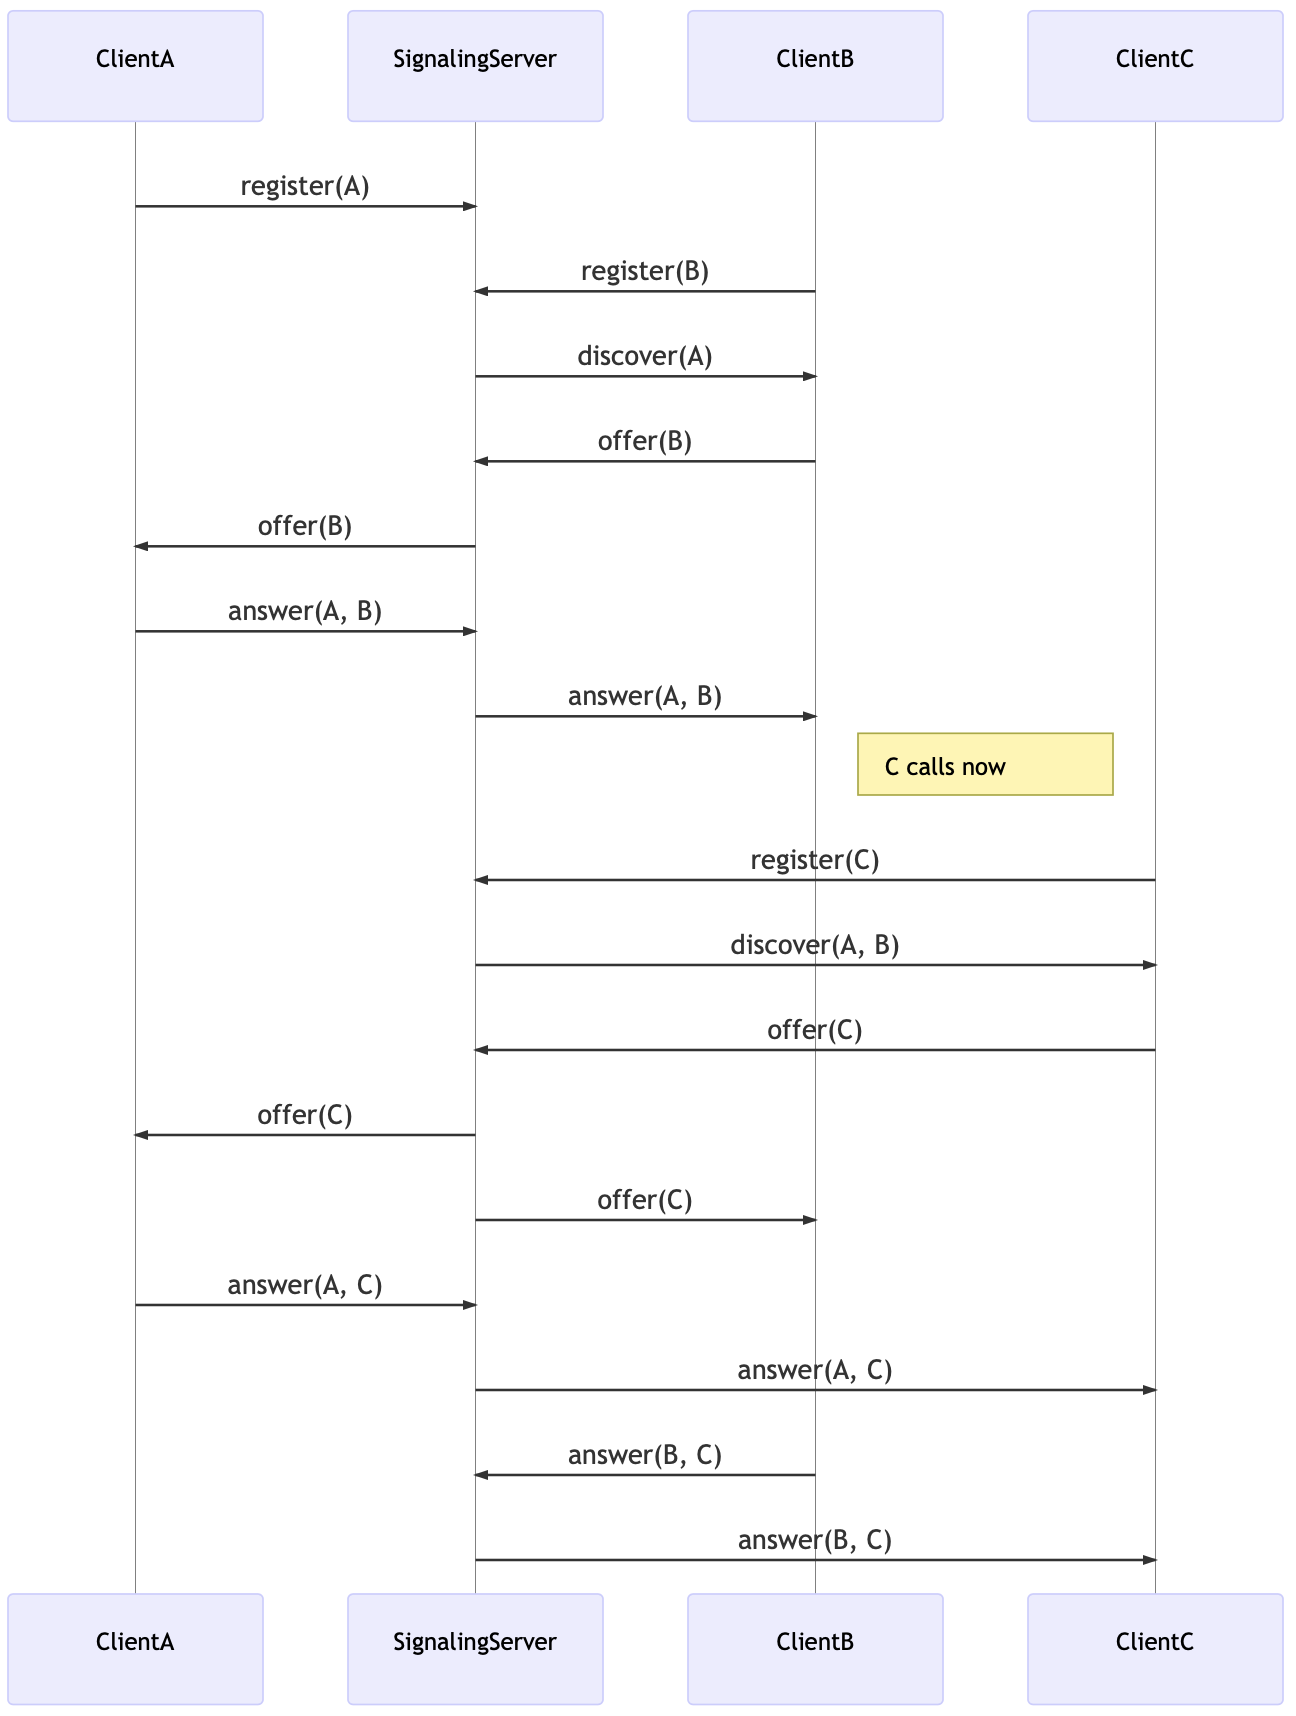
\includegraphics[scale=0.32]{cluster}
    \caption{Sequence diagram describing cluster construction}
    \label{fig:cluster}
\end{figure}

When a node comes online and seeks to become part of the cluster, it issues a \textit{register} call to our signaling server, which records the node's uuid as well as a socket for future communication with that node.

Every time a new node becomes registered, our signaling server broadcasts a \textit{discover} message to every registered node prior to that point with the uuid of the newly registered node.

Upon receiving a \textit{discover} message from the signaling server, the node then creates an SDP and forwards that via the signaling server to each newly discovered node.

Finally, upon receiving an \textit{offer} message from the signaling server, the receiving node forwards an \textit{answer} message along with its own SDP via the signaling server to the originator of the \textit{offer} message. At this point, every node in the cluster has the necessary information to establish peer to peer connections with each other and we can begin our Raft session.


\subsection{Signaling and STUN Servers}
In order to establish WebRTC connections, we built a simple signaling server that provided RPC and broadcast functionality to registered nodes. When communicating with our signaling server, clients must either provide a target uuid for their message to be forwarded or specify their intent to broadcast to all registered clients. Messaging with clients is conducted over web sockets. The server is implemented in Typescript and run via ts-node.

For gathering ICE candidates, we use publicly available STUN servers provided by Google.

\subsection{Raft}
To understand the intricacies of the Raft consensus algorithm, we built a from-scratch implementation in Typescript. For the sake of testing, we began by implementing Raft in a single process running in Node. This allowed us to easily construct scenarios described in the original Raft paper and quickly identify mistakes in our implementation. Once we felt that the fundamentals of our implementation were correct, we extracted our in-process RPC implementation and replaced it with RPC conducted over WebRTC. This approach has the added benefit of making our implementation somewhat platform agnostic. With minimal effort, we could provide RPC implementations over arbitrary transports and have versions of Raft that work in a browser using XMLHttpRequests, or in a headless context via Node and websockets.

Our specific implementation of Raft includes leadership election, appending entries, and client message forwarding. It does not implement cluster membership changes or log compaction.

\subsection{Chat Application}
To evaluate our implementation of Raft, we built a chat application that uses a replicated state machine to maintain chat history. One can envision this to be useful, as inconsistent chat histories can lead to confusion amongst participants.

Each client's chat history is comprised of only the committed entries in the log. Therefore, if a client becomes separated from the cluster, it will no longer be able to make progress on the log and any attempt to send messages will not be committed. If an offline client comes back online, any log entries committed by the rest of the cluster in the meantime will be replicated and the client will once again be able to send messages, as long as the cluster has quorum.

Because all communication is done directly between peers via WebRTC, no data is ever exposed to a centralized entity. Therefore, the peer-to-peer approach inherently protects a user's data better than in the centralized approach, where a user's data may become compromised as part of an attack on the managing entity.

\section{Challenges}

\subsection{Scalability}
To evaluate the latency of our implementation, we utilized Google's Puppeteer \cite{puppeteerwebsite} browser automation tooling to simulate Raft followers sending append RPCs sequentially for a span of 10 seconds. Measuring the number of sequential messages committed while varying the cluster size provided insight into how the implementation scales with larger clusters. We conducted 10 trials for each cluster size. The results of this evaluation can be seen in Figure \ref{fig:scale}.

\begin{figure}[t]
\centering
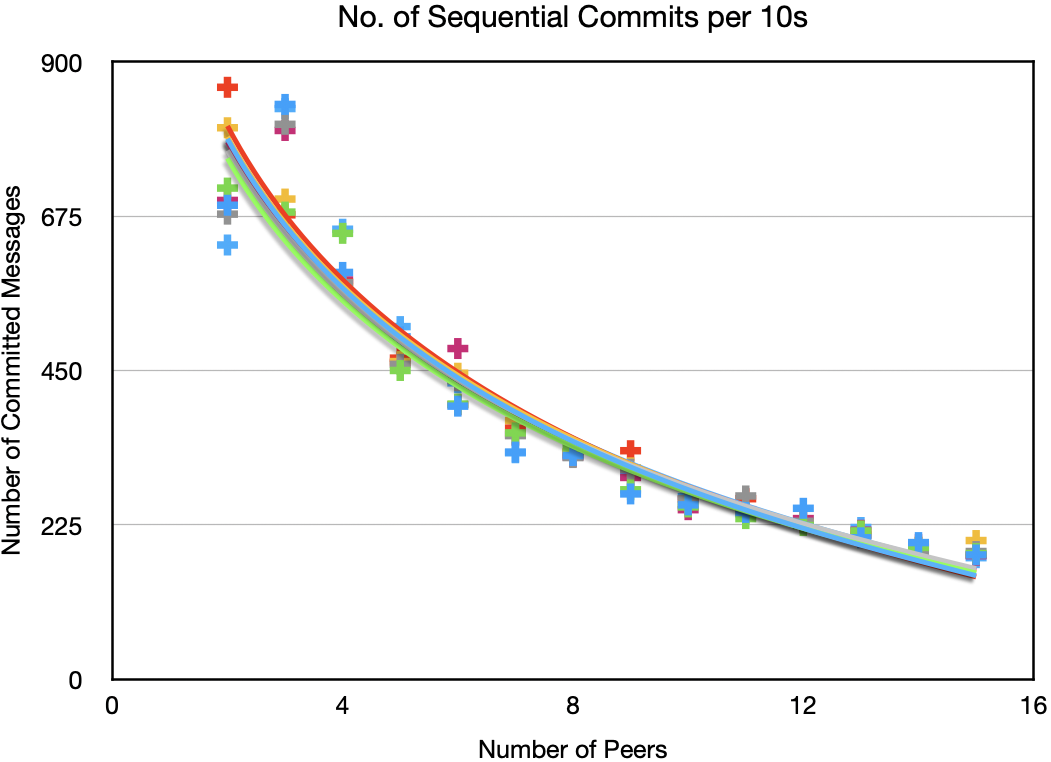
\includegraphics[scale=0.4]{performance}
\caption{Latency of system over cluster size. Conducted in Google Chrome on a 2016 MacBook Pro}
\label{fig:scale}
\end{figure}

We observed that the latency of the system degraded rapidly with an increase in cluster size before beginning to stabilize. To some degree, this is to be expected, as larger clusters require more messages to be sent between peers before log entries can be committed. However, we believe that the degraded performance with cluster size also reflects current browsers' limitations around maintaining large numbers of RTC connections.

\subsection{Byzantine Fault Tolerance}
Raft is not a byzantine fault tolerant consensus algorithm. However, the nature of achieving consensus in a user's browser exposes the algorithm to attacks from untrusted parties. While this can be mitigated with digital signing of RPCs, the cryptographic operations necessary would noticeably affect the latency of the system, as web browsers are still developing performant support for cryptography.

For these reasons, future additional work may want to evaluate the feasibility of byzantine fault tolerant algorithms in the browser context. Practical Byzantine Fault Tolerance (PBFT) \cite{pbftpaper} demonstrates byzantine fault tolerance with acceptable latency numbers for an application requiring responsiveness, such as chat. However, PBFT still relies on a concept of weak synchrony in which the network latency does not increase exponentially. This weak synchrony may not necessarily hold in less predictable environments as described in section 6.3.

\subsection{Predictability}
Many consensus-driven applications operate in highly controlled environments with certain guarantees on hardware and network performance. Achieving consensus on end-customer devices means that we cannot operate with any assumptions about the customer's computing conditions. In this context, the Raft consensus algorithm suffers, as it relies on tuned timeouts to determine when to begin leader election and cluster membership changes. For this project, the timeouts were manually chosen to reflect the author's network conditions. Future work may consider using dynamic timeouts as cluster members' network conditions change.

Honey Badger \cite{honeybadgerpaper} is a consensus algorithm designed with unpredictable network conditions in mind. However, its relatively high latency when compared with Raft and PBFT makes it less ideal for low-latency applications such as chat.

\subsection{Persistence}
In a centralized model, the problem of persisting data is handled by highly reliable data centers and servers. The decentralized model offers a challenge in that we cannot necessarily rely on clients to persist the log.

In our particular implementation of Raft in the browser, the closest we can achieve to persisting data is storing state using the browser local storage API. When recovering a session, a Raft node can seek out that stored state and use it to re-join a group. As described in section 4, a recovered node would initiate the WebRTC connection protocol and reconnect with all other live nodes.

In the event that a client deletes their persisted state, either by removing their browser or clearing their local browser data, that client would no longer be able to resume its role in the cluster. After a predetermined duration of not receiving RPCs from a deleted node, a live node in the cluster would initiate a cluster membership change that removes the stale node.


\section{Conclusion}
The centralized model for building consensus-based applications is often the go-to choice, as it provides more predictability and control for the implementor. However, this approach also requires trust from the end customer and incurs management costs for the providing entities. As network availability increases and consumer devices become more powerful, we believe there is significant potential in the decentralized model for building popular, reliable, trustworthy applications.

In this paper, we analyzed the viability of this decentralized approach by using accepted technologies to build a product with high expectations on reliability and latency. We provided a from-scratch implementation of the Raft consensus algorithm that uses WebRTC to facilitate direct communication between cluster peers. We used our Raft implementation to build and evaluate a chat application with consensus-based chat history. We found that Raft and WebRTC could be used to build a product that met customer expectations without exposing customer data to a centralized entity. We also found that the decentralized environment introduced new challenges around scalability, predictability of network conditions, and trustworthy persistence of customer data.

\printbibliography[type=book]


\end{document}
